\documentclass{article}

\usepackage{color,graphicx} 

\begin{document}
\title{GPU --- Architecture \& Programming \\ Assignment 1}
\author{Anirudhan Rajagopalan --- ajr619@nyu.edu}
\date{November 17, 2016}

\maketitle

\newpage
\section{List of optimizations}
\subsection{First GPU version}
Implemented with a kernel that takes the array and a prime number as arguments.  The kernel calculates its id and checks if its id is a perfect multiple of the prime number and also checks if it is not equal to the prime number.  If this condition matches, it sets the array to 1 and exits.

\textbf{Time for 10M}: Too long to wait (more than 30 minutes).  Killed the process.

\subsection{Second GPU version}

This version takes multiple prime numbers as inputs and does the same processing.
\begin{enumerate}
    \item When 8 primes are considered; Time = 5m, 20s
    \item When 128 primes are considered; Time = 1m, 32s
    \item When 1024 primes are considered; Time = 41.375 seconds
    \item When 2048 primes are considered; Time =  40 seconds
\end{enumerate}

While doing this testing, I also checked the code for branch divergence and other events that happens in the GPU\@.  From the summary output of nvcc, we can find that the majority of the time is spent in \textit{cudamemcopy}.
I tried to remove this by creating a <<<1,1>>> kernel that again creates multiple kernels for prime number processing.  
But this failed as I cannot compile this for the current cuda device I have.

\subsection{Reducing Branch Divergence}
\begin{enumerate}
    \item I tried reducing branch divergence by combining all exit cases into a single case.  This helped improved the performance by around 4 seconds.
    \item I also added conditions to check if a thread is processing a number which is already a non-prime.  This didn't improve the performance much.
    \item I added change to exit out of the for loop as soon as the number is found to be non-prime.  This helped in saving around 3 seconds.
\end{enumerate}

\section{Speed of GPU vs CPU}
\begin{figure}[ht!]
  \centering
  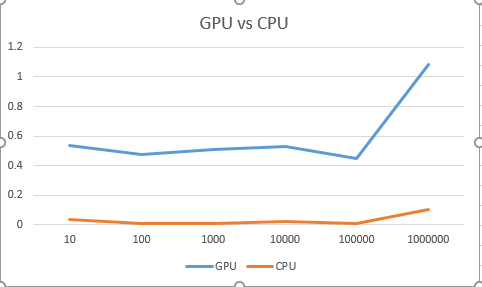
\includegraphics[width=1\textwidth]{gpuvscpu}
  \caption{GPU and CPU performance.\label{fig:gpuvscpu}}
\end{figure}

\section{Speedup for various values of N}
\begin{figure}[ht!]
  \centering
  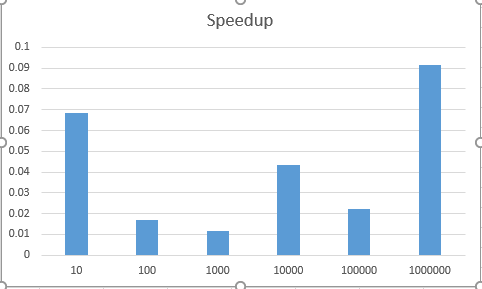
\includegraphics[width=1\textwidth]{speedup}
  \caption{Speedup.\label{fig:speedup}}
\end{figure}

\section{nvprof analysis}
\begin{figure}[ht!]
  \centering
  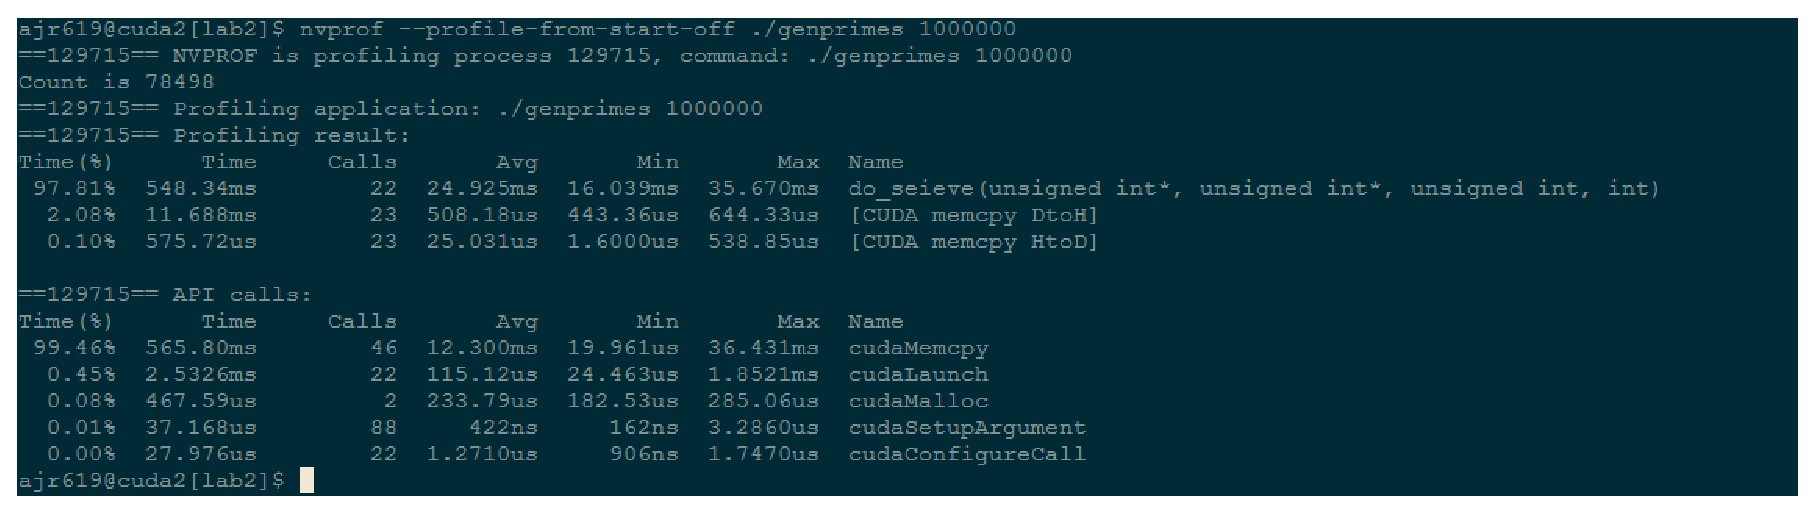
\includegraphics[width=1\textwidth]{nvprof}
  \caption{Basic nvprof profiling.\label{fig:speedup}}
\end{figure}

\begin{figure}[ht!]
  \centering
  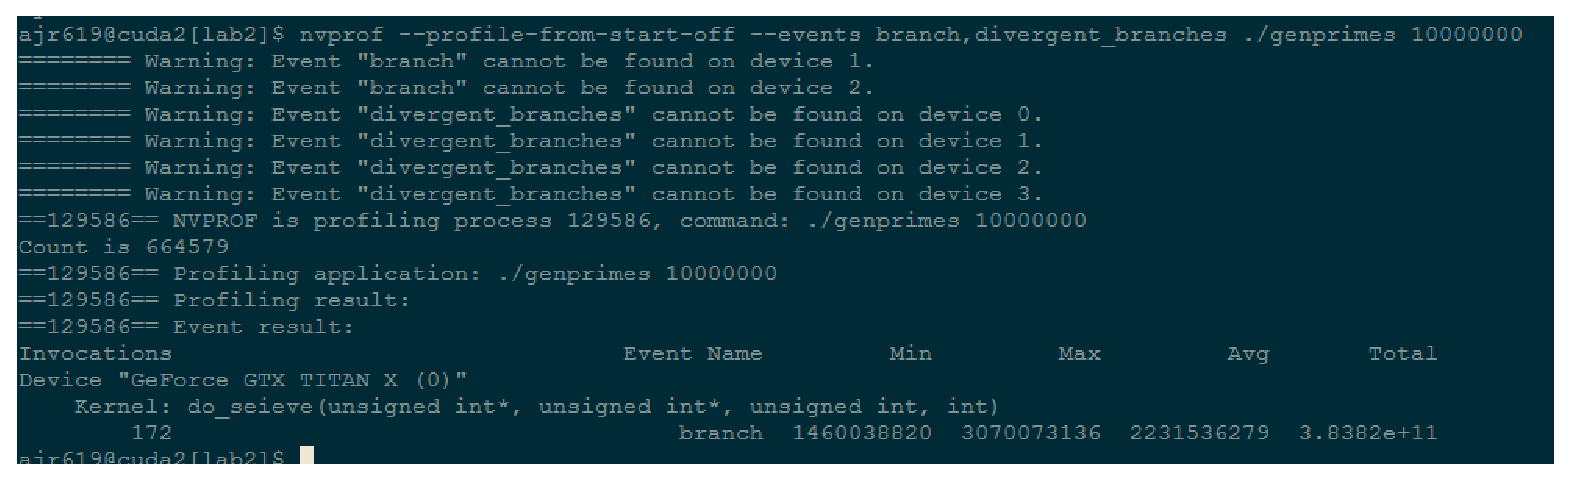
\includegraphics[width=1\textwidth]{branch_divergence}
  \caption{Branch Divergence.\label{fig:speedup}}
\end{figure}


\end{document}
